%% ---------------------------------------------------------------------------
%% intro.tex
%%
%% Introduction
%%
%% $Id: intro.tex 1477 2010-07-28 21:34:43Z palvarado $
%% ---------------------------------------------------------------------------

\chapter{Introduction}
\label{chp:intro}

\section{Artifacts in live video streaming}
\label{sec:intro_artifacts}

Modern streaming services are fundamental instruments in today's industries, institutions, and every day life. Live video conferencing and streaming services became the principal medium of communication for a large sector of local and global communities during the recent COVID-19 pandemic, thus exemplifying the crucial role that these services now have. Current advances in network speed and digital technology have enabled these services to become commonplace in professional, academic, and recreational contexts. Therefore, there has been increased interest in ensuring a high quality of experience (QoE) for these services.

One of the main issues affecting the QoE of video conferencing and live streaming services are video artifacts \cite{Vranjes2018, Korhonen2018}. Video artifacts, or simply artifacts, are defined as distortions in the images displayed to the user with respect to the original captured images \cite{Greengrass2009}. According to \cite{Vranjes2018}, artifacts are primarily caused by errors or loss of data in the transmission of the video over the network, or by losses caused during video compression.

Figure \ref{fig:lossy_system} illustrates the basic structure of a lossy video system. In order to send video through a network, a video is encoded into network packets, then it is sent through a transmission channel where the losses occur, and finally it is decoded into video with artifacts. Figure \ref{fig:frame_comparison} compares two versions of the same image. Figure \ref{fig:frame_comparison.a} contains no video artifacts and Figure \ref{fig:frame_comparison.b} contains video artifacts due to packet loss.

\begin{figure} [!h]
  \centering
  
  \includegraphics{lossy_system}
  
  \caption{Lossy video transmission system}
  \label{fig:lossy_system}

\end{figure}

\begin{figure} [!h]
  \centering
  
  \begin{subfigure}[t]{0.49\textwidth}
    \centering
    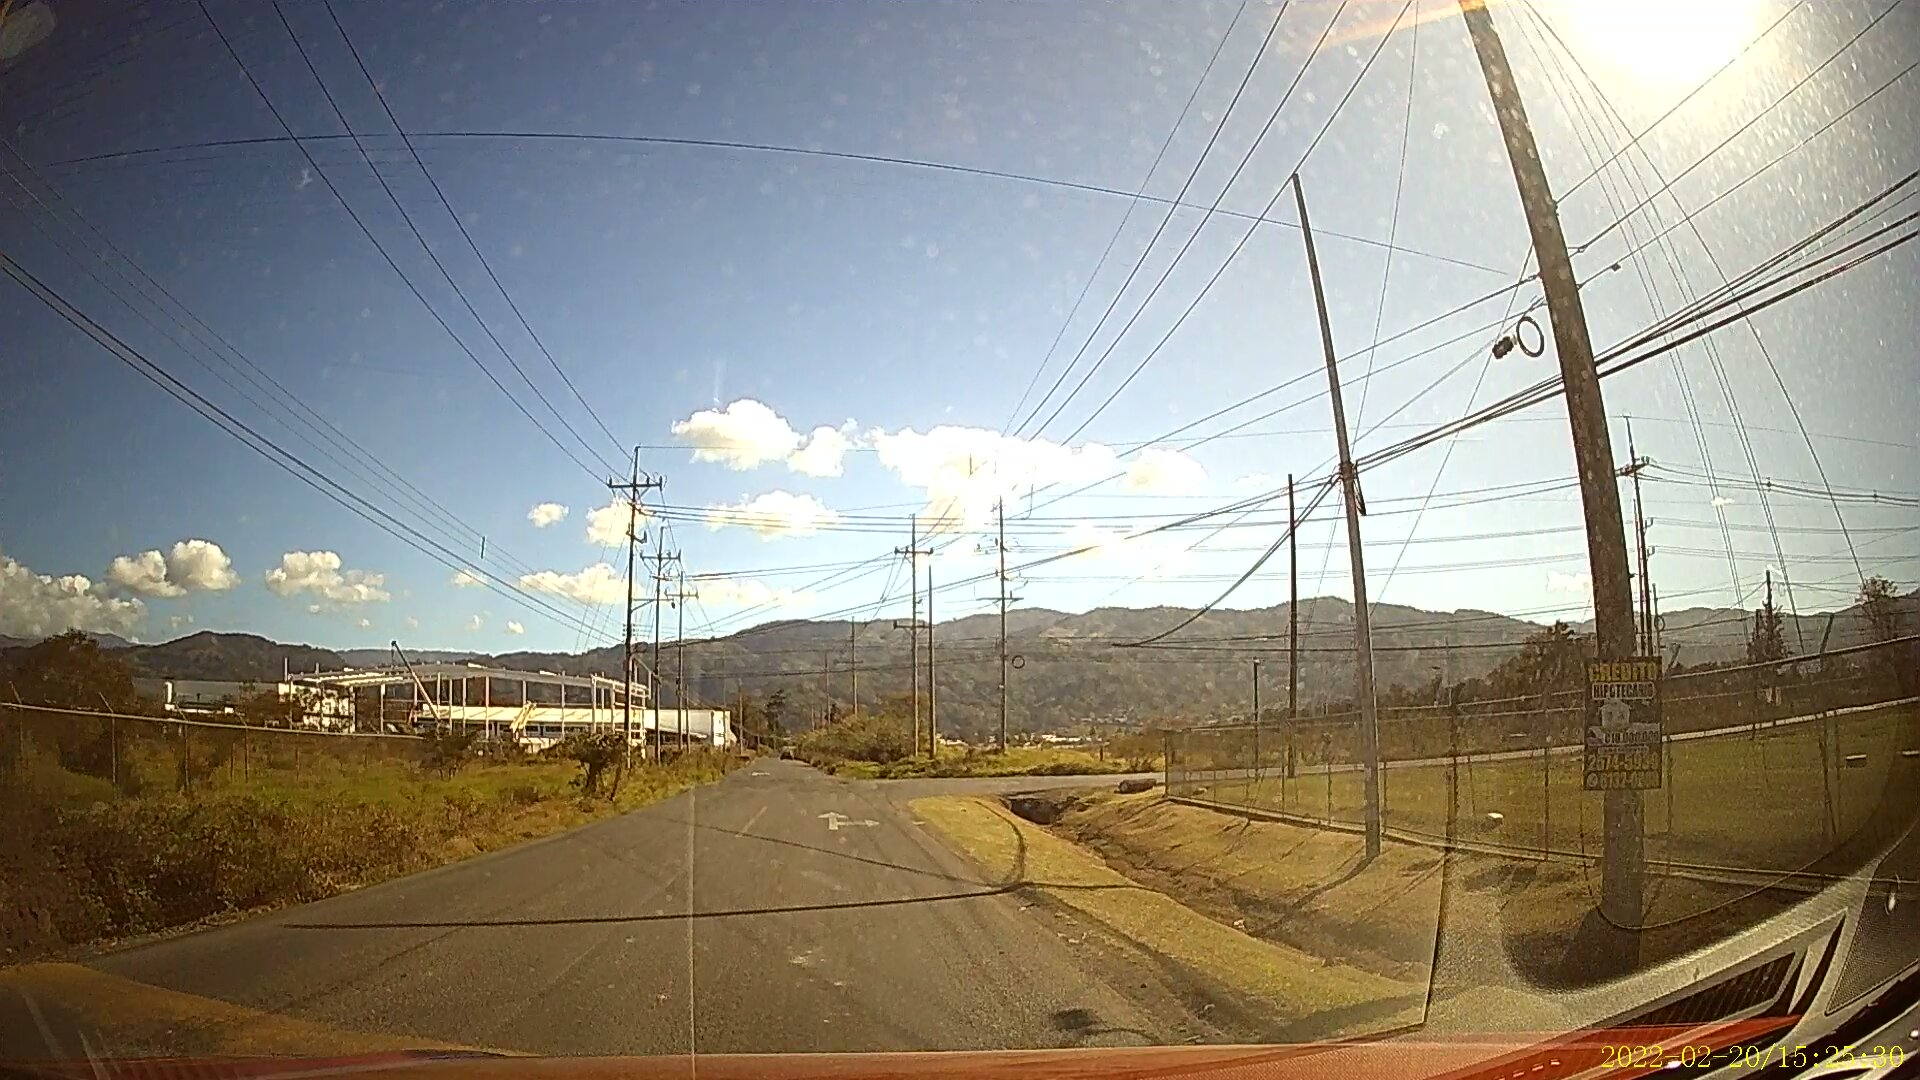
\includegraphics[width=\textwidth]{imgs_27}
    \caption{Frame with no video artifacts}
    \label{fig:frame_comparison.a}
  \end{subfigure}
  \hfill
  \begin{subfigure}[t]{0.49\textwidth}
    \centering
    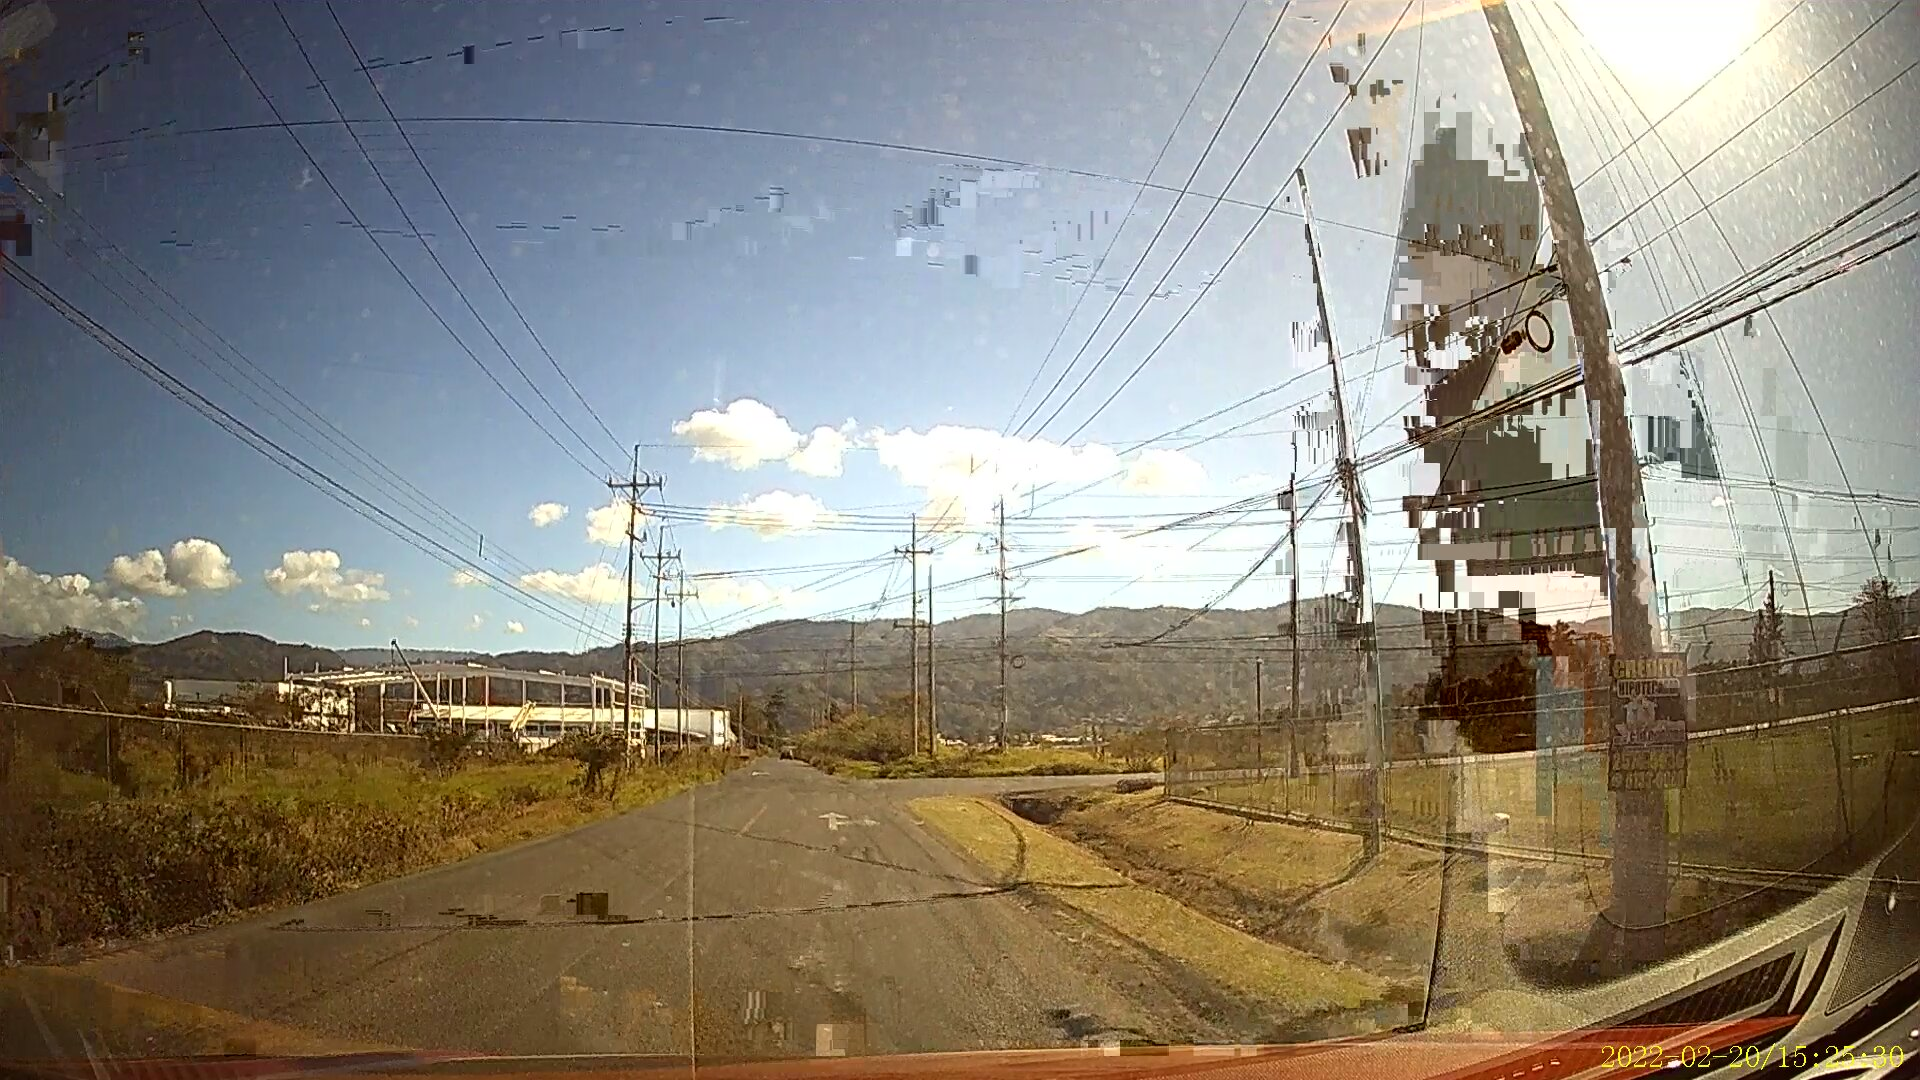
\includegraphics[width=\textwidth]{imgs_with_loss_27}
    \caption{Frame with video artifacts due to packet loss.}
    \label{fig:frame_comparison.b}
  \end{subfigure}
  
  \caption{Comparison between a video frame with no artifacts and a video frame with artifacts caused by random packet losses.}
  \label{fig:frame_comparison}

\end{figure}

There are methods to correct transmission errors in the transport layer or even in the video syntax layer of the OSI model \cite{Sanyal2021}. In these cases, information is available on how the video packets are encoded, which simplifies the task of error detection and correction. However, when the user only has the decoded and decompressed information, it is necessary to use methods for artifact detection and correction that only rely on the raw video information, such as those of \cite{Vranjes2018, Sanyal2021,Goodall2019}. These methods are referred to as ``no-reference methods''.

Video artifacts result in loss of information from the original video. In video conferencing and live streaming applications, it is not possible to recover the lost data without affecting the user's QoE. In order to correct video artifacts, no-reference methods must restore the lost data. The process of restoring unknown areas of an image is called ``video inpainting'' \cite{Li2022, Zhou2021}. Video inpainting, or simply inpainting, is commonly used to remove the presence of objects in a video or image, but can also be used to reconstruct areas of an image affected by video artifacts \cite{Dong2023, Brenes2022}.

Modern inpainting algorithms use machine learning models. Many inpainters use ``transformers'' \cite{Li2022, Zhou2021, Liu2021}, which are machine learning models with outstanding results for signal restoration tasks, but they are slow and require signficant processing power. GPUs and other hardware accelerators are used in order to optimize the performance of these models.

Inpainting models such as \cite{Li2022,Brenes2022} require binary masks to identify the areas to be reconstructed. For this reason, the location of video artifacts must be detected and binary masks must be generated and then used in the image restoration stage.

The studies \cite{Greengrass2009, Glavota2016} classify the various types of artifacts generated by packet loss. These studies also describe the statistical properties of video artifacts. For example, certain video artifacts tend to have high-contrast vertical and horizontal edges that can be detected by high-pass filters. In the MPEG and H.26x video compression standards, the pixels of an image are grouped into ``macroblocks'', which are groups of $16 \times 16$ pixels in the image. Losses of packets containing macroblock information result in artifacts with well-defined edges \cite{Vranjes2019, Glavota2018}.

The artifact detection methods from \cite{Vranjes2018, Glavota2018} focus on filtering algorithms that do not involve machine learning. These methods can process standard definition video at 30 frames per second without GPU acceleration, but they oversimplify the characteristics of video artifacts and fail to perform well on the artifact detection task. The detectors of \cite{Goodall2019, Rajasekar2020} use neural network classifiers. These methods generalize better than filtering algorithms, but they require GPU accelerators in order to achieve comparable framerates with the filtering algorithms.

\section{The Video Restoration System}
\label{sec:intro_disptec}

The dispTEC2 project developed a Video Restoration System for the Nvidia Jetson TX2 Embedded System using DeepLearning. The Jetson TX2 machine has a 256 CUDA-core GPU, a Quad-core ARM CPU, and a Dual-core Denver CPU. The dispTEC2 team found that the Denver CPU was not useful to the project, thus the Jetson TX2 machine was effectively a 4-core machine.

The resulting system is composed of an Artifact Detection System and an Inpainter System \cite{Brenes2022}. The system is capable of processing a video frame by frame. For each frame it simulates randomly linear H264 packet losses, it generates a binary detection mask based on the ground truth artifact measure, and then it feeds the mask along with the lossy frame into an inpainter transformer to produce a restored frame. Brenes \cite{Brenes2022} optimized the Inpainter System through a series of arquitectural redesigns and through the use of the CUDA accelerated PyTorch. He finally concluded that the system reaches a framerate from 0.8 to 1.67 frames per second on the Nvidia Jetson TX2.

However, this system supposes the existence of an Artifact Detector System that can generate binary detection masks from the input video with artifacts.

\section{The Artifact Detector Problem}
\label{sec:intro_problem}

The Video Restoration System concluded without a proper artifact detector. The artifact detector was expected to run on the ARM 4-core CPU alone, not interfering with the CUDA-accelerated inpainting model and possibly decrease the inpainting speed. As a first approach, the system used the Packet Loss Detection Algorithm (PLDA) from \cite{Vranjes2018}. When testing the algorithm inside a gstreamer element \cite{gstreamer}, the algorithm could process a 720p video at $23$ frames per second.  After extensive testing of the algorithm using the Non-dominated Sorting Genetic Algorithm (NSGA-II) \cite{Deb2002}, the dispTEC2 team found no suitable parameters that allowed the detector to perform well on the detection task. 

The dispTEC2 team also developed a second artifact detection approach based on Random Decision Forests (RDF) \cite{Breiman2001}. In this approach, the RDF classifiers operated directly on each raw video frame and could achieve slightly better detection results than a random classifier. This classifier was trained on 200 frames from a training dataset containing only 2 video content types. When testing the RDF approach inside a gstreamer element, the algorithm could process 720p video at $27$ frames per second.

These results suggested that the RDF classifers were capable of learning artifact detection from the raw frame information. These results also suggested that the algorithm could be optimized to reach a framerate of $30$ frames per second.

\todo{Find PLDA framerate and metrics}
\todo{Find RDF framerate and metrics}

\section{Art-FD}
\label{sec:intro_detector}

The dispTEC2 Video Restoration System is designed to restore video with artifacts frame by frame. The system has two main components: the Artifact Detection System and the Inpainting System. Figure \ref{fig:restoration_system_steps} displays the inner structure of the Video Restoration System.

The Artifact Detection System takes the frames with artifacts and generates binary detection masks. These masks divide each image into macroblocks and then assign a value to all macroblocks that are detected to contain video artifacts. The Inpainting System takes the frames with artifacts and the detection masks. It then generates the restored video frames by removing the macroblocks marked as artifacts and inpainting the removed regions.

\begin{figure} [!h]
  \centering
  
  \includegraphics{video_inpainter_steps}
  
  \caption{Video restoration procedure. }
  \label{fig:restoration_system_steps}

\end{figure}

This work proposes a new ``ARTiFact Detector'' (Art-FD) based on Random Decision Forests, which aims to improve over the dispTEC2 detection system by expanding the training dataset, redesigning and optimizing the feature extraction strategy, and replacing the RDF backend with the optimized Ranger C++ Core Library.

Random Decision Forests are subject to overfitting when trained with small, highly self correlated datasets \cite{Breiman2001}. Art-FD expands the dataset with diverse video content in order to reduce the RDF detector overfitting.

The dispTEC2 RDF detector learned from raw image data. However, the feature extraction strategy is improved by considering some of the statistical properties of artifacts described in \cite{Vranjes2019, Glavota2018}. Art-FD filters the raw image data to detect high contrast vertical and horizontal borders, then generates 132 statistical features from the filtered results.

Random Decision Forests agregate the results of a set of independent Decision Tree Classifiers. The dispTEC2 RDF library ran the individual classifers consecutivelly. In contrast, the Ranger C++ Core Library runs the individual classifiers concurrently in separate threads. Art-FD replaces the dispTEC2 RDF backend with Ranger in order to improve both training and detection speed.

\section{Project Objectives and Document Structure}
\label{sec:intro_objectives}

The aim of this project is to develop Art-FD, a real-time Artifact Detection System that generates binary detection masks from video with artifacts. The project shares two general aspects with the dispTEC2 project: it focuses on video artifacts produced by decoding H264 packet loss and it aims to run on an NVIDIA Jetson TX2 without using the GPU. Art-FD aims to improve over the dispTEC2 system in three ways:

\begin{enumerate}
  \item it shall be trained on a dataset with at least 18 video content types and 200 frames each,
  \item it shall achieve a minimum of 70\% in both precision and recall detection metrics, and
  \item it shall achieve a framerate of 30 frames per second.
\end{enumerate}

The first contribution of Art-FD is to expand the training dataset by obtaining new video material and generating the dataset input-output pairs. The choice of 18 content types is meant to reduce overfitting in the trained models over the original set of 2 content types. Brenes provides a ground truth generation tool \cite{Brenes2022}, which is used as a starting point for the creation of dataset outputs. The final dataset should contain 18 video content types with at least 3 different illumination types.

The second contribution of Art-FD is implementing the training procedure, the feature selection and the replacement of the RDF backend. These steps are aimed at improving the precision and recall detection performance metrics over 70\%. These metrics are meant to improve over the precision of 69\% and 58\% of the dispTEC2 RDF classifier.

The third contribution of Art-FD is optimizing the feature selection and detection procedures in order to achieve real-time performance. Art-FD should process over 30 frames per second, which means that each frame detection should last under 33 ms. This goal is meant to improve over the 27 frames per second of the dispTEC2 RDF classifier.

This work is structured as follows. Chapter \ref{ch:marco} explores several theoretical concepts used in the development of Art-FD. Chapter \ref{ch:solucion} describes Art-FD in detail. Chapter \ref{chp:results} discusses Art-FD's results. Chapter \ref{chp:conclusions} summarizes the project's main conclusions, as well as future work related to Art-FD and dispTEC2's Video Restoration System.
